\chapter{Introduction}

The software development lifecycle has evolved from just developing software systems to developing robust and reliable software systems. The reliability of software depends on its ability to perform its functions according to the given specifications and to handle exceptional or abnormal cases [1].
\paragraph{}
The Design by Contract (DbC) methodology provides software developers with the ability to construct reliable software systems without much extra effort. DbC is useful throughout the process of building software, from analysis and design to implementation, documentation, debugging, and even project management[1]. A contract is made up of pre-conditions and post-conditions, which are used for making assertions in the given system. These different conditions define a relationship between the client (end user) and the supplier (software developer). This relationship is said to be broken if any of the conditions do not hold true.



\section{Contract Conditions}

\begin{itemize}
\item A precondition is a condition that should hold true when a call is made to the method. If this condition fails, then the call to the method fails and blame can be assigned to the client for providing incorrect input values.
\item A postcondition is a condition on a method that should hold true when the execution of the method successfully completes. If it does not, then it can be asserted that something went wrong during execution and blame can be assigned to the supplier for providing an erroneous system that does not work according to the given specifications.
\item An invariant is something that needs to be true from the start until the end (throughout the execution), of the call to the method.
\end{itemize}

Given these constructs, if an application completes the execution without the failure of any of the pre or post conditions provided in the contract, then we can assert that the written code is doing what it is meant for and nothing less or nothing extra [1].
However, the quality of the assertion made depends on how well the contracts conditions are written. 

\section{A Contract for an ATM System}

An example of an ATM system given below illustrates the use of contracts.
In this example, the ATM system is our supplier and a person using the ATM system is the client. Let's suppose the supplier provides two functions for depositing and withdrawing money.
\begin{itemize}
\item Withdraw :
Here the client is obliged to enter a non-zero amount to be withdrawn from his/her account, which also should be less than the balance in his/her account. This obligation for the client forms the precondition of our contract.
Now, once the client provides the correct amount to be withdrawn, the supplier (ATM system) is obliged to update the balance by decrementing the input amount from it. This obligation for the supplier forms the postcondition of our contract.
\linebreak
\begin{figure}[htb]
\centering
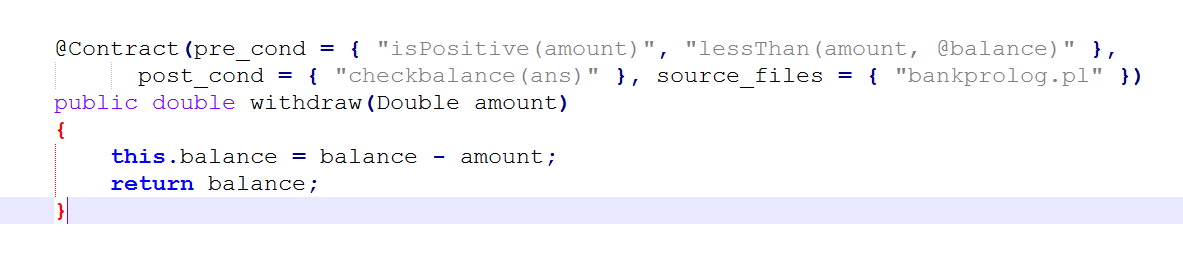
\includegraphics[width=0.5\textwidth]{images/WithdrawContractExample.PNG}
\caption{Contract for Withdraw method.} 
\label{fig:WithdrawContract}
\end{figure}

\newpage

\item Deposit :
Here the client is obliged to insert the amount to be deposited, which should be non-zero and less than the maximum limit allowed (let's say 1500\$). This forms the precondition for the contract of the Deposit function.
On successful execution of Deposit function, the supplier is obliged to increase the balance by the deposited amount. This forms the postcondition of the contract.
\linebreak
\begin{figure}[htb]
\centering
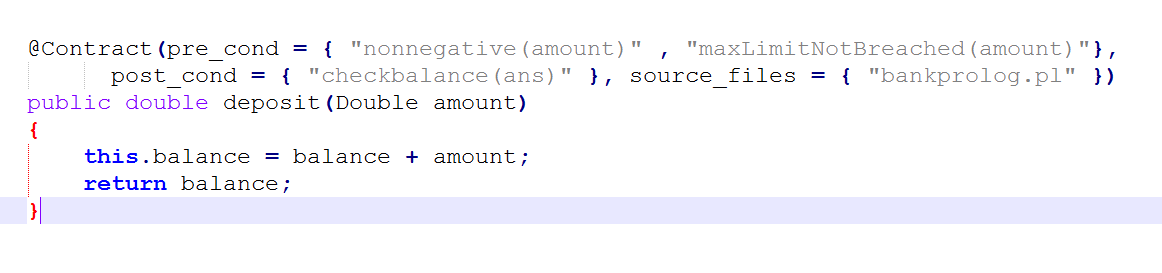
\includegraphics[width=0.5\textwidth]{images/DepositContract.PNG}
\caption{Contract for Deposit method.} 
\label{fig:DepositContract}
\end{figure}  
      
\end{itemize}


\section{Prolog for Contracts}
From above two examples function defined in the contract annotation as preconditions and postconditions form queries to a Prolog program. This Prolog program acts as database file for the library. When these queries are executed against these rules given in the Prolog program, it results into a boolean assertion which helps library evaluate if all the contracts were successful or if they had some failures.   
Figure.~\ref{fig:PrologProgram} below shows an example of Prolog file that can be used with the bank ATM example illustrated in above section. Logical syntax of the Prolog code makes it very easy to understand and implement these rules.

\begin{figure}[htb]
\centering
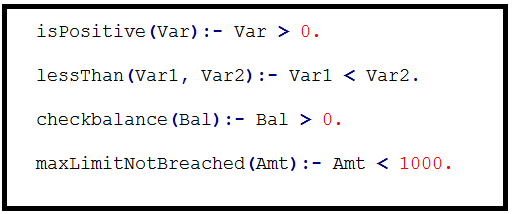
\includegraphics[width=0.5\textwidth]{images/PrologDatabase.PNG}
\caption{Prolog File with Contract Rules.} 
\label{fig:PrologProgram}
\end{figure} 